
\documentclass[article,a4paper]{IEEEtran}
\usepackage{lipsum}
\usepackage[backend=biber]{biblatex}
\usepackage{graphicx}

\addbibresource{refs.bib}
\title{IIoT - Industry Internet of Things with Industry 4.0}
\author{
\IEEEauthorblockN{Anton Odén}\\
\IEEEauthorblockA{Dept. of Maths and Computer Science\\Karlstad University\\
651 88 KARLSTAD, Sweden}\\
anton.oden@outlook.com
}

\begin{document}

\maketitle
    \begin{abstract}
    The winner in manufacturing if most effective at allocating resources, producing and distributing produce. Behind all this is human activity that has been automated over time. From the first revolution with machinery automating producing parts, to second electrifing revolution giving benefits to all parts. Then digital age further streamlined the parts nessaary in manufacturing. All it's about is information to make action. The faster the allocation of information and the computing act to make action can happen the more effective the manufacturing.
    \end{abstract}
    
    \section{Introduction}
    In this article I will further discuss how Industry 4.0 (IoT, AI and Cyber physical systems) can be integrated into lean production systems. Some impacts on efficiency and flexibility. What challenges that needs to be taken into consideration and future prospecs with references to the papers "Industry 4.0 impacts on lean production" \cite{Impact_Lean_Prod} and "How virtualization, decentralization and network chand the manufacturing landscape: An Industry 4.0 perspective" \cite{Change_Man_Landscape}

    \section{Background}
    Industry 4.0 is the reference to the fourth revolution of manufacturing industry that is the implementation of cyber-physical systems, internet of things, big data, analytics and artificial intelligence. But to give some historic reference: The first revolution was when industry started to use machines powered by other energysources than manpower. Second revolution was the electrifing of industries. Electric power made industry location less dependent on position compared to first revolution that was dependent on power to be generated at the same location as it was used. Electric power compared to steam could be transported. Together with electric power communication over large distances was made possible. Making huge impacts on logistics. Third industry revolution is the digitalization of industry which we still are in today and it's has been going on since 1960. Digital record-keeping, digitilized and automated processes, robotics has made efficience improvements unto manufacturing and logistics. \newline\newline
    The fourth industry revolution is the connectivity between all parts of manufacturing, tranforming this data into information and the analytics of this information to make informed and/or automatic decisionmaking. Connecting Cloud, Enterprise Resource Planning(ERP), manufacturing excecuting software (MES), Supervisory Control and Data Acquisition (SCADA), Programming logic controllers (PLC)/ Human-Machine interfaces (HMI) \cite{industry4.0} with Supply chain management (SCM), Autonomous mobile robots (AMRs), Predictive Maintenance systems (PMS) and quality management systems (QMS). The list could be made many pages on all the systems that could be used by a manufacturer.
    \newline\newline
    Exploitation of Internet of Things (IoT) getting data direcly from plant floor all these mentioned systems could react at an instant. For example if a manufacturing order halts cause of defects on incoming material was noticed inline. The ERP could recalculate planned delivery, MES could feed next manufacturing order, maybe reorder the manufacturing queue. AMRs could be feeding the line with different material without human interaction inbetween. All these systems becomes gets high value from data from the plant floor. The system for collecting, informatize and analyze data between enterprise systems and our IoT is refered to as Cyber-physical systems (CPS). These systems are being able to make real-time decisions reacting to psysical events and even predict physical events beforehand. Adding articifial intelligence to these systems may enhanced these prediction capabilities.
    \newline\newline
    Lean production is often given origin rights to Toyota production system. 5S, Kaizen, Just-in-Time, Continuous improvement, Standardisation etc. Where aim is to deliver produce while avoiding waste at the value chain. 
    \begin{figure}
        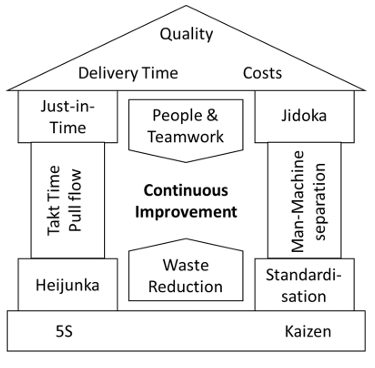
\includegraphics{HouseofToyota.png} 
        \caption{House of Toyota Manufacturing Systems}
        \label{fig1:House of Toyota Manufacturing System}   
    \end{figure}
    \ref{fig1:House of Toyota Manufacturing System}
    The shown House of Lean Production is the symbol for the Lean Production principles. The triangle roof emlematizes the systamic focus on customer oriented key performance indicators (KPI) for quality, delivery time and cost. The basic approach is a continuous improvement of production. Industry 4.0 with IoT could bring lots of benefits within the Lean production standard. \cite{Impact_Lean_Prod}
    \newline\newline
    
    \section{Integration of Technologies}
    The concept of internet of things is that all is connected. Connecting expensive machines with expensive servers is not what is meant. But the things that are referenced to are small microprocessors combined with sensors and actuators that could in theory be made to collect and control from anything. Making anything a part of the Internet (or intranet more prefferable). Temperature and humidity (TH) is something that in many processes affects results in manufacturing and factories sets up routines and may have machines that halts work if thresholds reached. But thanks to cheap sensors the production could have overview of the TH in all areas of production and letting crucial processes subscribe to this information production could be halted and the data could also be saved and analysed in later quality essesment. A customer complaint could for the manufacturer be linked to bad TH and the manufacturer could then have traceability on all serial numbers produced under same circumstances. The ERP and MES systems may react instant to the shift in TH and switch production focus for the day if not the automatic systems for bringing TH to wanted levels is successful. 

    Making the collection of data, actuating actions and analysing automatic cyber-physical systems emerges where the systems in the self are able to make decisions based on set algorithms. Adding on top of this we have machine learning technologies that further could enhanced decicion making for the systems. Big Data and analytics which is closely related to AI is a subjects within industry which the servey in \cite{Impact_Lean_Prod} sees highest possible impact on most areas in lean production. Out of 11 TPS principles Kaizen, Just-in-Time, Jidoka, Heijunka, Standardisation, Takt time, Waste reduction is impacted the most. 

    Another integration in lean production is virtual and augmented reality. Augmented reality could help operators to follow the lean production principles. Giving operators tips in their viewing field what to do and what to expect on a working station. THe augumented reality could have different levels with first level being for beginners giving clear instruction on what to do, what to expect on a station and when to consult a senior. To later levels where data is given upfront where a senior is able to decide what to do based on the data. AI in turn could be trained when being attached to a senior operator augumented reality. If the senior operator picks up a screwdriver. The augumented reality for a beginner operator will tell him/her to pick up the screwdriver. watching time to do different montagesteps could be recorded and AI could give tips based on this data to do montage in different steps. This are some examples why the industry accoring to \cite{Impact_Lean_Prod} sees highest impacts on lean principles 5S, Kaizen, Standardisation, Man-machine separation and teamwork.  

    According to  sensors and actuators could have an high impact on TPS Heijunka. 

    \section{Impact of efficiency and flexibility}

    \section{IIoT - Industry Internet of Things}
    The idea is that the more data is accumilated the better decisions could be made. The collection of data is partly done via IoT(Internet of Things). And by things not only meaning physical devices. Every database, software, machine, sensor and actuaters are connected prefferable via a comon namespace. All things in the industry publishes data to that comon namespace and other things are able to subscribe to the comon namespace to be able to make decisions. Combining all the avaibale data, making it available to use and tranforming the data into information to take automatic action on. That is Industry 4.0. And to make that happen. The internt of things is neccesary.  
    

    \section{Cyber-physical system}

    \section{Lean Production}
    A paper by published 2017 in Braunschweig Germany \cite{Impact_Lean_Prod} discuss the impacts that IIoT could have on the well established 
    



    \section{No more paper}
    \section{Realtime metrics}
    \section{Big data analytics}
    \cite{Change_Man_Landscape}
    
    dawdad
    \section{Conclusion}

\printbibliography
\end{document}